\chapter{Fenchel Conjugates and Newton's Method}
% \documentclass[draft,11pt]{article}
%\documentclass[11pt]{article}
%%  RASMUS  packages
\usepackage{blindtext}
\usepackage[usenames,dvipsnames,svgnames,table]{xcolor}
\usepackage{enumitem}
\usepackage{caption}
\usepackage{placeins}
\usepackage{graphicx}

\usepackage{fancybox}
\usepackage{hyperref}

\usepackage{amsmath,amsfonts,amsthm,amssymb,xcolor}
% \let\amsboldsymbol\boldsymbol % if you want to see the bad
% boldsymbol for comparison
\usepackage{bm} % fixes boldsymbol
\usepackage{nicefrac}
\usepackage{float}

% switched to algorithm2e in lecture 9
% \usepackage{algorithm} %ctan.org\pkg\algorithms
% \usepackage{algorithmic}
% \usepackage{algorithmicx}
% \usepackage[noend]{algpseudocode}

\newtheorem{theorem}{Theorem}[section]
\newtheorem{corollary}[theorem]{Corollary}
\newtheorem{lemma}[theorem]{Lemma}
\newtheorem{observation}[theorem]{Observation}
\newtheorem{proposition}[theorem]{Proposition}
\newtheorem{invariant}[theorem]{Invariant}
\newtheorem{claim}[theorem]{Claim}
\newtheorem{fact}[theorem]{Fact}
\newtheorem{assumption}[theorem]{Assumption}
\newtheorem{warning}[theorem]{Warning}
\newtheorem{conjecture}[theorem]{Conjecture}

\newtheorem{pseudotheorem}{Pseudotheorem}[section]
\newtheorem{pseudoclaim}[theorem]{Pseudoclaim}


\theoremstyle{definition}
\newtheorem{definition}[theorem]{Definition}
\newtheorem{remark}[theorem]{Remark}

\newtheorem*{theorem*}{Theorem}
\newtheorem*{corollary*}{Corollary}
\newtheorem*{conjecture*}{Conjecture}
\newtheorem*{lemma*}{Lemma}
\newtheorem*{thm*}{Theorem}
\newtheorem*{prop*}{Proposition}
\newtheorem*{obs*}{Observation}
\newtheorem*{definition*}{Definition}
\newtheorem*{example}{Example}
\newtheorem*{remark*}{Remark}
\newtheorem*{rec*}{Recommendation}

\newenvironment{fminipage}%
  {\begin{Sbox}\begin{minipage}}%
  {\end{minipage}\end{Sbox}\fbox{\TheSbox}}

\newenvironment{algbox}[0]{\vskip 0.2in
\noindent 
\begin{fminipage}{6.3in}
}{
\end{fminipage}
\vskip 0.2in
}


\let\muchl\ll

\def\pleq{\preccurlyeq}
\def\pgeq{\succcurlyeq}
\def\pge{\succ}
\def\ple{\prec}

\def\Approx#1{\approx_{#1}}

%\def\Span#1{\textbf{Span}\left(#1  \right)}
\def\bvec#1{{\mbox{\boldmath $#1$}}}


\newcommand\congestion{\mathit{cong}}

\def\prob#1#2{\mbox{Pr}_{#1}\left[ #2 \right]}
\def\pvec#1#2{\vec{\mbox{P}}^{#1}\left[ #2 \right]}
\def\expec#1#2{{\mathbb{E}}_{#1}\left[ #2 \right]}
\def\var#1{\mbox{\bf Var}\left[ #1 \right]}

\def\defeq{\stackrel{\mathrm{def}}{=}}
\def\setof#1{\left\{#1  \right\}}
\def\sizeof#1{\left|#1  \right|}


\def\trace#1{\mathrm{Tr} \left(#1 \right)}

\def\floor#1{\left\lfloor #1 \right\rfloor}
\def\ceil#1{\left\lceil #1 \right\rceil}

\def\dim#1{\mathrm{dim} (#1)}
\def\sgn#1{\mathrm{sgn} (#1)}

\def\union{\cup}
\def\intersect{\cap}
\def\Union{\bigcup}
\def\Intersect{\bigcap}

\def\abs#1{\left|#1  \right|}

\def\norm#1{\left\| #1 \right\|}
\def\smallnorm#1{\| #1 \|}

\newcommand\grad{\boldsymbol{\nabla}}
\newcommand\D[2]{D#1[#2]}

\newcommand*\diff{\mathop{}\!\mathrm{d}}
\newcommand*\Diff[1]{\mathop{}\!\mathrm{d^#1}}

\newcommand\ip[1]{\left< #1 \right>}


\newcommand{\sym}[1]{\mathrm{sym} (#1)}



\def\calC{\mathcal{C}}
\def\calD{\mathcal{D}}
\def\calE{\mathcal{E}}
\def\calF{\mathcal{F}}
\def\calG{\mathcal{G}}
\def\calL{\mathcal{L}}
\def\calS{\mathcal{S}}
\def\calT{\mathcal{T}}
\def\calM{\mathcal{M}}

\newcommand\calDD{\boldsymbol{\calD}}

\newcommand\DDelta{\boldsymbol{\mathit{\Delta}}}
\newcommand\Ppsi{\boldsymbol{\mathit{\Psi}}}
\newcommand\PPsi{\boldsymbol{\mathit{\Psi}}}
\newcommand\ppsi{\boldsymbol{\mathit{\psi}}}
\newcommand\pphi{\boldsymbol{\mathit{\phi}}}
\newcommand\PPhi{\boldsymbol{\Phi}}
%\newcommand\Llambda{\boldsymbol{\mathit{\Lambda}}}
\newcommand\LLambda{\boldsymbol{\mathit{\Lambda}}}
\newcommand\PPi{\boldsymbol{\Pi}}

\newcommand\ppi{\boldsymbol{\pi}}
\newcommand\cchi{\boldsymbol{\chi}}
\newcommand\aalpha{\boldsymbol{\alpha}}
\newcommand\bbeta{\boldsymbol{\beta}}
\newcommand\ggamma{\boldsymbol{\gamma}}
\newcommand\ddelta{\boldsymbol{\delta}}

\newcommand\rrho{\boldsymbol{\rho}}
\newcommand\xxi{\boldsymbol{\xi}}
%\newcommand\cchi{\boldsymbol{\chi}}

\newcommand\er{R_{\text{eff}}}


\def\aa{\pmb{\mathit{a}}}
\newcommand\bb{\boldsymbol{\mathit{b}}}
\newcommand\cc{\boldsymbol{\mathit{c}}}
\newcommand\dd{\boldsymbol{\mathit{d}}}
\newcommand\ee{\boldsymbol{\mathit{e}}}
\newcommand\ff{\boldsymbol{\mathit{f}}}
\renewcommand\gg{\boldsymbol{\mathit{g}}}
\newcommand\ii{\boldsymbol{\mathit{i}}}
\newcommand\jj{\boldsymbol{\mathit{j}}}
\newcommand\kk{\boldsymbol{\mathit{k}}}
\renewcommand\ll{\boldsymbol{\mathit{l}}}
\newcommand\pp{\boldsymbol{\mathit{p}}}
\newcommand\qq{\boldsymbol{\mathit{q}}}
\newcommand\bs{\boldsymbol{\mathit{s}}}
\newcommand\nn{\boldsymbol{\mathit{n}}}
\newcommand\rr{\boldsymbol{\mathit{r}}}
\renewcommand\ss{\boldsymbol{\mathit{s}}}
\def\tt{\boldsymbol{\mathit{t}}}
\newcommand\uu{\boldsymbol{\mathit{u}}}
\newcommand\vv{\boldsymbol{\mathit{v}}}
\newcommand\ww{\boldsymbol{\mathit{w}}}
\newcommand\yy{\boldsymbol{\mathit{y}}}
\newcommand\zz{\boldsymbol{\mathit{z}}}
\newcommand\xx{\boldsymbol{\mathit{x}}}

\newcommand\veczero{\boldsymbol{0}}
\newcommand\vecone{\boldsymbol{1}}

\newcommand\matzero{\boldsymbol{0}}
\newcommand\matone{\boldsymbol{1}}

\newcommand{\matlow}{\boldsymbol{\mathit{{\mathcal{L}}}}}
\newcommand{\matlowtil}{\boldsymbol{\mathit{\widetilde{\mathcal{L}}}}}
\newcommand{\matlowhat}{\boldsymbol{\mathit{\widehat{\mathcal{L}}}}}

\newcommand{\matup}{\boldsymbol{\mathit{{\mathcal{U}}}}}


\renewcommand\AA{\boldsymbol{\mathit{A}}}
\newcommand\BB{\boldsymbol{\mathit{B}}}
\newcommand\CC{\boldsymbol{\mathit{C}}}
\newcommand\DD{\boldsymbol{\mathit{D}}}
\newcommand\EE{\boldsymbol{\mathit{E}}}
\newcommand\GG{\boldsymbol{\mathit{G}}}
\newcommand\HH{\boldsymbol{{H}}}
\newcommand\II{\boldsymbol{\mathit{I}}}
\newcommand\JJ{\boldsymbol{\mathit{J}}}
\newcommand\KK{\boldsymbol{\mathit{K}}}
\newcommand\NN{\boldsymbol{\mathit{N}}}
\newcommand\MM{\boldsymbol{\mathit{M}}}
\newcommand\LL{\boldsymbol{\mathit{L}}}
\newcommand\PP{\boldsymbol{\mathit{P}}}
\newcommand\RR{\boldsymbol{\mathit{R}}}
\renewcommand\SS{\boldsymbol{\mathit{S}}}
\newcommand\TT{\boldsymbol{\mathit{T}}}
\newcommand\UU{\boldsymbol{\mathit{U}}}
\newcommand\WW{\boldsymbol{\mathit{W}}}
\newcommand\VV{\boldsymbol{\mathit{V}}}
\newcommand\XX{\boldsymbol{\mathit{X}}}
\newcommand\YY{\boldsymbol{\mathit{Y}}}



\newcommand\MMtil{\boldsymbol{\mathit{\tilde{M}}}}
\newcommand\AAtil{\boldsymbol{\mathit{\tilde{A}}}}
\newcommand\BBtil{\boldsymbol{\mathit{\tilde{B}}}}
\newcommand\LLtil{\boldsymbol{\mathit{\tilde{L}}}}
\newcommand\MMtilde{\boldsymbol{\mathit{\tilde{M}}}}
\newcommand\XXtil{\boldsymbol{\mathit{\tilde{X}}}}

\newcommand\AAn{\boldsymbol{\mathcal{A}}}
\newcommand\ZZ{\boldsymbol{\mathit{Z}}}

\newcommand\AAhat{\boldsymbol{\widehat{\mathit{A}}}}
\newcommand\AAapprox{\boldsymbol{\widetilde{\mathit{A}}}}
\newcommand\DDhat{\boldsymbol{\widehat{\mathit{D}}}}
\newcommand\DDapprox{\boldsymbol{\widetilde{\mathit{D}}}}
\newcommand\LLhat{\boldsymbol{\widehat{\mathit{L}}}}
\newcommand\LLapprox{\boldsymbol{\widetilde{\mathit{L}}}}
\newcommand\MMhat{\boldsymbol{\widehat{\mathit{M}}}}
\newcommand\MMapprox{\boldsymbol{\widetilde{\mathit{M}}}}
\newcommand\ZZhat{\boldsymbol{\widehat{\mathit{Z}}}}

\newcommand\DDtil{\boldsymbol{\widetilde{\mathit{D}}}}

\newcommand\fftil{\boldsymbol{\tilde{\mathit{f}}}}
\newcommand\sstil{\boldsymbol{\tilde{\mathit{s}}}}
\newcommand\xxtil{\boldsymbol{\tilde{\mathit{x}}}}
\newcommand\yytil{\boldsymbol{\tilde{\mathit{y}}}}
\newcommand\wwtil{\boldsymbol{\tilde{\mathit{w}}}}

\newcommand\ddeltatil{\boldsymbol{\tilde{\mathit{\delta}}}}


\newcommand\Otil{\widetilde{O}}

\newcommand\xhat{{\hat{{x}}}}
\newcommand\uhat{{\hat{{u}}}}
\newcommand\uuhat{\boldsymbol{\mathit{\hat{u}}}}
\newcommand\vhat{{\hat{{v}}}}
\newcommand\what{{\hat{{w}}}}

\newcommand\Ghat{{\widehat{{G}}}}
\newcommand\GGhat{\boldsymbol{\widehat{G}}}

\newcommand\Ehat{{\widehat{{E}}}}


\newcommand\R{\mathbb{R}}
\newcommand\N{\mathbb{N}}

\newcommand\ffhat{\boldsymbol{\hat{\mathit{f}}}}

\newcommand\cchat{\boldsymbol{\widehat{\mathit{c}}}}
\newcommand\sshat{\boldsymbol{\mathit{\widehat{s}}}}
\newcommand\xxhat{\boldsymbol{\mathit{\widehat{x}}}}
\newcommand\yyhat{\boldsymbol{\widehat{\mathit{y}}}}
\newcommand\xxbar{\overline{\boldsymbol{\mathit{x}}}}
\newcommand\yybar{\overline{\boldsymbol{\mathit{y}}}}
\newcommand\xxstar{{\boldsymbol{\mathit{x}}^{*}}}
\newcommand\yystar{{\boldsymbol{\mathit{y}}^{*}}}

\let\ggreater\gg
\newcommand\bwInt{\boldsymbol{{\mathit{w}}}}
\newcommand\bw{\boldsymbol{\mathit{w}}}
\DeclareMathOperator{\Cong}{\mathtt{cong}}
\DeclareMathOperator{\dist}{\mathtt{dist}}


\newcommand\ffbar{\overline{\boldsymbol{\mathit{f}}}}


\newcommand\ddeltabar{\boldsymbol{\bar{\mathit{\delta}}}}
\newcommand\ddeltahat{\boldsymbol{\hat{\mathit{\delta}}}}



\newcommand\energy{\mathcal{E}}


\newcommand{\todo}[1]{{\bf \color{red} TODO: #1}}
\newcommand{\todolow}[1]{{\bf \color{orange} TODOLOW: #1}}

\newcommand{\richard}[1]{{\bf \color{green} Richard: #1}}
\newcommand{\rasmus}[1]{{\bf \color{olive} Rasmus: #1}}
\newcommand{\ahad}[1]{{\bf \color{olive} Ahad: #1}}

\newcommand{\expct}[2]{{}\mathop{\mathbb{E}}_{#1}\left[#2\right]}
\newcommand{\E}[1]{\mathop{{}\mathbb{E}}\left[#1\right]}
%% https://tex.stackexchange.com/questions/56765/getting-the-expectation-symbol-to-behave-like-sum-instead-of-sigma
%% extra {} inside mathop gives nicer (standard) vertical placement of E
\newcommand{\Var}[1]{\mathop{{}Var}\left[#1\right]}
\newcommand{\Ex}[1]{{}\mathop{\mathbb{E}}_{#1}}
\newcommand\tr{\mathrm{Tr}}


%%%%% LINEAR ALGEBRA

\newcommand{\schurto}[2]{\ensuremath{\textsc{Sc}\!\left[#1\right]_{#2}}}
% \newcommand{\schurto}[2]{\ensuremath{\textsc{Sc}\left[#1\right]_{#2}}}

%{$\textsc{Sc}\left[#1\right]_{#2}$}
% \newcommand{\schurto}[2]{\textsc{Sc}\left(#1, #2\right)}
%\newcommand{\schurto}[2]{\left[{#1}\right]_{\to #2}}
\renewcommand{\sc}[2]{\schurto{#1}{#2}}

%transpose
\newcommand{\trp}{\top}

%pseudoinverse
\newcommand{\pinv}{+}


\newcommand{\proj}{\PPi}

\DeclareMathOperator{\nnz}{nnz}

\DeclareMathOperator*{\argmin}{arg\,min}
\DeclareMathOperator*{\argmax}{arg\,max}
\DeclareMathOperator*{\val}{val}

\DeclareMathOperator*{\diag}{diag}
\DeclareMathOperator*{\Span}{span}

%\DeclareMathOperator*{\ker}{ker}
\DeclareMathOperator*{\im}{im}

%%%%% LAYOUT

\newenvironment{tight_enumerate}{
\begin{enumerate}
 \setlength{\itemsep}{2pt}
 \setlength{\parskip}{1pt}
}{\end{enumerate}}
\newenvironment{tight_itemize}{
\begin{itemize}
 \setlength{\itemsep}{2pt}
 \setlength{\parskip}{1pt}
}{\end{itemize}}
\newenvironment{tight_description}{
\begin{description}
 \setlength{\itemsep}{2pt}
 \setlength{\parskip}{1pt}
}{\end{description}}

\newcommand*{\vertbar}{\rule[-1ex]{0.5pt}{2.5ex}}
\newcommand*{\horzbar}{\rule[.5ex]{2.5ex}{0.5pt}}

%Basics
\newcommand{\new}[1]{{\em #1\/}}		% New term (set in italics).

\newcommand{\boxwidth}{\dimexpr\linewidth-2em\relax}

\newcommand{\boxdef}[1]
{
\fbox{
\begin{minipage}{\boxwidth}
\begin{definition}
{#1}
\end{definition}
\end{minipage}
}
}

\newcommand{\boxthm}[1]
{
\fbox{
\begin{minipage}{\boxwidth}
\begin{theorem}
{#1}
\end{theorem}
\end{minipage}
}
}

\newcommand{\boxfact}[1]
{
\fbox{
\begin{minipage}{\boxwidth}
%\begin{theorem*}
\emph{{#1}
%\end{theorem*}
}
\end{minipage}
}
}

%\newcommand{\handout}[5]{
  \noindent
  \begin{center}
  \framebox{
    \vbox{
            \hbox to 6.30in { {\bf Advanced Graph Algorithms and Optimization} \hfill #2 }
            \vspace{5mm}
            \hbox to 6.30in { {\Large \hfill #5  \hfill} }
            \vspace{3mm}
            \hbox to 6.30in { {\em #3 \hfill #4} }
    }
  }
  \end{center}
  \vspace*{4mm}
}

\newcommand{\lecture}[4]{\handout{#1}{#2}{#3}{Lecture #1}{#4}}
\newcommand{\homework}[3]{\handout{#1}{#2}{#3}{Problem Set #1}}
\newcommand{\gradedhomework}[3]{\handout{#1}{#2}{#3}{Graded Homework #1}}
\newcommand{\sect}[3]{\handout{#1}{#2}{#3}{Section #1}}




% 1-inch margins, from fullpage.sty by H.Partl, Version 2, Dec. 15, 1988.
\topmargin 0pt
\advance \topmargin by -\headheight
\advance \topmargin by -\headsep
\textheight 8.9in
\oddsidemargin 0pt
\evensidemargin \oddsidemargin
\marginparwidth 0.5in
\textwidth 6.5in

\parindent 0in
\parskip 1.5ex
 
%\usepackage{amsmath}
%\usepackage{amssymb}
%\usepackage{amsthm}
%\usepackage{graphicx}
%\usepackage{float}
%\usepackage[ruled,vlined]{algorithm2e}
%\SetKwBlock{Repeat}{repeat}{}

%%% for this lecture
%\newcommand\numberthis{\addtocounter{equation}{1}\tag{\theequation}}
%\newcommand\st{~\mathrm{s.t.}~}
%\newcommand\ttau{\boldsymbol{\tau}}
%\newcommand{\df}{\mathrm{d}}
%\def\hcalE{\hat{\mathcal{E}}}

%%%% ADD MACROS HERE
% feel free to add more macros here

%\begin{document}

\sloppy
%\lecture{13 --- Wednesday, May 20th}{Spring 2020}{Rasmus Kyng, Scribe:
%  Hongjie Chen}{
%Karush-Kuhn-Tucker Conditions, Fenchel Conjugates, Newton's Method
%}
\section{Lagrange Multipliers and Convex Duality Recap}
Recall the convex optimization program we studied last chapter,
\begin{align*}
  \min\quad & \calE(\yy) \\
  \text{s.t.}\quad  & \AA\yy = \bb \numberthis \label{eq:primal} \\
              & \cc(\yy) \leq \veczero,
\end{align*}
where $\calE(\yy): S \rightarrow \R$ is defined on a subset $S \subseteq \R^n$, $\AA \in \R^{m\times n}$
and $\cc(\yy)$ is a vector of constraints $\cc(\yy) = \left(c_i(\yy)\right)_{i \in [k]}$.
For every $i \in [k]$ the function $c_i: S \rightarrow \R$ is convex. We call (\ref{eq:primal}) the primal (program) and denote its optimal value by $\alpha^*$.

The associated Lagrangian is defined by
\[
  L(\yy, \xx, \ss) = \calE(\yy) + \xx^T(\bb-\AA\yy) + \ss^T\cc(\yy).
\]
where $\xx \in \R^m$, $\ss \in \R^k$ are dual variables. The dual (program) is given by
\begin{equation}
  \label{eq:dual}
  \max_{\substack{\xx, \ss \\ \ss \geq 0}} \quad L(\xx,  \ss)
\end{equation}
whose optimal value is denoted by $\beta^*$. The dual is always a convex optimization program even though the primal is non-convex.
The optimal value of the primal (\ref{eq:primal}) can also be written as
\begin{equation}\label{eq:alpah}
  \alpha^* = \inf_{\yy} \sup_{\xx; \ss\geq\veczero} L(\yy, \xx, \ss),
\end{equation}
where no constraint is imposed on the primal variable $\yy$.
The optimal value of the dual (\ref{eq:dual}) is
\begin{equation}\label{eq:beta}
  \beta^* = \sup_{\xx; \ss\geq\veczero} \inf_{\yy} L(\yy, \xx, \ss).
\end{equation}
Note the only difference between (\ref{eq:alpah}) and (\ref{eq:beta}) is that the positions of ``inf" and ``sup" are swapped.
The weak duality theorem states that the dual optimal value is a lower bound of the primal optimal value, i.e.\ $\beta^* \leq \alpha^*$.

The Slater's condition for (\ref{eq:primal}) open domain $S$ requires the existence of a \emph{strictly feasible} point, i.e.\ there exists $\yytil\in S$ s.t.\ $\AA\yytil = \bb$ and $\cc(\yytil) < \veczero$.
This means that the strictly feasible point $\yytil$ lies inside the
interior of the set $\{\yy : \cc(\yy) \leq \veczero\}$ defined by the
inequality constraints.
If the domain $S$ is not open, Slater's condition also requires that a
strictly feasible point is in the relative interior of $S$ (NB:
when $S$ is open, $S$ is equal to its relative interior).
The strong duality theorem says that Slater's condition implies strong
duality, $\beta^* = \alpha^*$.

We were also introduced to the KKT conditions, and we saw that for our
convex programs with continuously differentiable objective and
constraints functions, when the domain is open, the conditions are sufficient to
imply strong duality and primal-dual optimality of the points that
satisfy them, KKT $\implies$ `$(\yy,\xx,\ss)$ primal-dual optimal and
we have strong duality'.
Finally, we saw that when strong duality holds,
KKT must hold at the
primal-dual optimal solutions.

\textbf{In summary:} \emph{Slater's condition $\implies$ strong duality}
and \emph{strong duality $\iff$ KKT}.

\begin{example}
  In Chapter~\ref{cha:maxflow2}, we gave a combinatorial proof of the min-cut max-flow
  theorem, and showed that the min-cut program can be expressed as a
  linear program. Now, we will use the strong duality theorem to give
  an alternative proof, and directly find the min-cut linear program
  is the dual program to our maximum flow linear program.

  We will assume that Slater's condition holds for our primal
  program.
  Since scaling the flow down enough will always ensure that
  capacity constraints are strictly satisfied i.e.\ $\ff < \cc$, the
  only concern is to make sure that non-negativity constraints are satisfied.
  This means that there is an $s$-$t$ flow that sends a non-zero flow
  on every edge.
  In fact, this may not always be possible, but it is
  easy to detect such edges and remove them without changing the value
  of the program: an edge $(u,v)$ should be removed if there is no
  path $s$ to $u$ or no path $v$ to $t$. We can identify all such
  edges using a BFS from $s$ along
  the directed edges and a BFS along reversed directed edges from $t$.

\begin{align*}
    \min_{\begin{subarray}{c} F\in\R \\ \BB\ff=F\bb_{s,t} \\ \veczero\leq\ff\leq\cc \end{subarray}} -F
    &= \min_{F;\ff\geq\veczero} \max_{\xx;\ss\geq\veczero} -F + \xx^\trp(F\bb_{s,t}-\BB\ff) + (\ff-\cc)^\trp\ss \\
    & \text{(Slater's condition $\implies$ strong duality)} \\
    -\max_{\begin{subarray}{c} F\in\R \\ \BB\ff=F\bb_{s,t} \\ \veczero\leq\ff\leq\cc \end{subarray}} F
    &= \max_{\xx;\ss\geq\veczero} \min_{F;\ff\geq\veczero} F(\bb_{s,t}^\trp\xx-1) + \ff^\trp(\ss-\BB^\trp\xx) -\cc^\trp\ss \\
    &= \max_{\begin{array}{c} \xx;\ss\geq\veczero \\ \bb_{s,t}^\trp\xx=1 \\ \ss\geq\BB^\trp\xx
             \end{array}} -\cc^\trp\ss
  \end{align*}
  Thus switching signs gives us
    \begin{align*}
    \max_{\begin{subarray}{c} F\in\R \\ \BB\ff=F\bb_{s,t} \\ \veczero\leq\ff\leq\cc \end{subarray}} F
    &= \min_{\begin{array}{c} \xx;\ss\geq\veczero \\ \bb_{s,t}^\trp\xx=1 \\ \ss\geq\BB^\trp\xx
    \end{array}} \cc^\trp\ss \numberthis \label{eq:min-cut-max-flow}
  \end{align*}
  The LHS of (\ref{eq:min-cut-max-flow}) is exactly the LP formulation
  of max-flow, while the RHS is exactly the LP formulation of min-cut.
  Note that we treated the ``constraint'' $ \veczero\leq\ff$ as a
  restriction on the domain of $\ff$ rather than a constraint with a
  dual variable associated with it.
  We always have this kind of flexibility when deciding how to compute
  a dual, and some choices may lead to a simpler dual program than others.
\end{example}

\section{Fenchel Conjugates}
In this section we will learn about Fenchel conjugates. This is a
notion of dual function that is closely related to duality of convex
programs, and we will learn more about how dual programs behave by
studying these functions.

\begin{definition}[Fenchel conjugate]
  Given a (convex) function $\calE:S\subseteq\R^n\to\R$, its \emph{Fenchel conjugate} is a function $\calE^*:\R^n\to\R$ defined as
  \[ \calE^*(\zz) = \sup_{\yy\in S} \langle \zz,\yy \rangle - \calE(\yy). \]
\end{definition}

\begin{remark}
  $\calE^*$ is a convex function whether $\calE$ is convex or not, since $\calE^*(z)$ is pointwise supremum of a family of convex (here, affine) functions of $z$.
\end{remark}

In this course, we have only considered convex functions that are
real-valued and continuous and defined on a convex domain. For any such $\calE$, we have $\calE^{**} = \calE$,
i.e.\ the Fenchel conjugate of the Fenchel conjugate is the original
function.
This is a consequence of the Fenchel-Moreau
theorem, which establishes this under slightly more general conditions.
We will not prove this generally, but as part of
Theorem~\ref{thm:conjugate} below, we sketch a proof under more restrictive assumptions.

\begin{example}
  Let $\calE(\yy) = \frac{1}{p}\|\yy\|_p^p ~(p>1)$. We want to evaluate its Fenchel conjugate $\calE^*$ at any given point $\zz\in\R^n$. Since $\calE$ is convex and differentiable, the supremum must be achieved at some $\yy$ with vanishing gradient
  \[ \grad_{\yy}\langle \zz,\yy^* \rangle - \grad\calE(\yy^*) = \zz - \grad\calE(\yy^*) = \matzero \iff \zz = \grad\calE(\yy^*). \]
  It's not difficult to see, for all $i$,
  \[ \zz(i) = \sgn{\yy(i)}|\yy(i)|^{p-1}. \]
  Then,
  \begin{align*}
    \calE^*(\zz)
    &= \langle \zz,\yy \rangle - \calE(\yy) \\
    &= \sum_{i}|\zz(i)|^{\frac{1}{p-1}+1} - \frac{1}{p}|\zz(i)|^{\frac{p}{p-1}} \\
    & (\text{define } q \st \frac{1}{q}+\frac{1}{p} = 1) \\
    &= \frac{1}{q} \|\zz\|_q^q.
  \end{align*}
\end{example}

More generally, given a convex and differentiable function $\calE:S\to\R$, if there exists $\yy\in S$ s.t.\ $\zz = \grad\calE(\yy)$, then $\calE^*(\zz) = (\yy^*)^\trp\grad\calE(\yy^*)-\calE(\yy^*)$.
The Fenchel conjugate and Lagrange duality are closely related, which
is demonstrated in the following example.


\begin{example}
  Consider a convex optimization program with only linear constraints,
  \begin{align*}
    \min_{\yy\in\R^n}\quad & \calE(\yy) \\
    \st\quad  & \AA\yy = \bb
  \end{align*}
  where $\calE:\R^n\to\R$ is a convex function and $\AA\in\R^{m\times n}$.
  Then the corresponding dual program is
  \begin{align*}
    \sup_{\xx\in\R^n}\inf_{\yy\in\R^n} \calE(\yy) + \xx^\trp(\bb-\AA\yy)
    &= \sup_{\xx\in\R^n}\bb^\trp\xx - \sup_{\yy\in\R^n} \left(\xx^\trp\AA\yy - \calE(\yy)\right) \\
    &= \sup_{\xx\in\R^n}\bb^\trp\xx - \calE^*(\AA^\trp\xx) \\
  \end{align*}
\end{example}

\begin{theorem}[Properties of the Fenchel conjugate]
  \label{thm:conjugate}
  Consider a strictly convex function ${\calE : S \to \R}$ where $S \subseteq
  R^n$ is an open convex set. When $\calE$ is differentiable with a Hessian
  that is positive definite everywhere and its gradient $\grad \calE$
is surjective onto
  $\R^n$, we have the following three properties:
  \begin{enumerate}
  \item $\grad\calE(\grad\calE^*(\zz))=\zz$ \text{and} $\grad\calE^*(\grad\calE(\yy)) = \yy$ \label{enu:gradmap}
  \item $(\calE^*)^* = \calE$, i.e.\ the Fenchel conjugate of the \label{enu:doubleconj}
      Fenchel conjugate is the original function.
  \item $\HH_{\calE^*}(\grad\calE(\yy)) = \HH_{\calE}^{-1}(\yy)$ \label{enu:hessianmap}
  \end{enumerate}
\end{theorem}

\begin{figure}[H]
\begin{mdframed}
  \centering
%  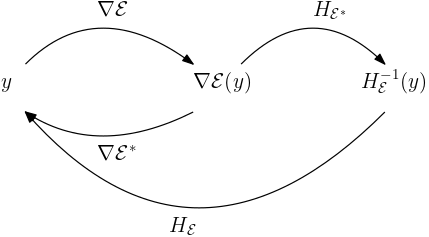
\includegraphics[width=0.5\linewidth]{fig/Fenchel_conjugate.png}
\begin{center}
\begin{tabular}{ c c c }
 primal point $\yy$
  & $  \begin{matrix}
    \xrightarrow{\grad_{\yy} \calE }{} \\
     \xleftarrow{\grad_{\zz} \calE^* }{}
   \end{matrix}$ &
                   dual point $\zz$ \\
  \\
 gradient $\grad_{\yy} \calE(\yy) = \zz$  & & gradient $\grad_{\zz}
                                              \calE^*(\zz) = \yy$ \\
  \\
 Hessian $\HH_{\calE}(\yy) = \HH_{\calE^*}^{-1}(\zz) $ & & Hessian $\HH_{\calE^*}(\yy) = \HH_{\calE}^{-1}(\yy)$
\end{tabular}
\end{center}
  \caption{Properties of Fenchel conjugate}
  \label{fig:fenchel}
\end{mdframed}
\end{figure}

\begin{proof}[Proof sketch]
  \emph{Part \ref{enu:gradmap}.}
  Because the gradient $\grad_{\yy}\calE$ is surjective onto $\R^n$,
  given any $\zz \in \R^n$, there exists a $\yy$ such that $\grad
  \calE(\yy) = \zz$.  Let $\yy(\zz)$ be a $\yy$ s.t. $\grad
  \calE(\yy) = \zz$.
  It can be shown that because $\calE$ is strictly convex, $\yy(\zz)$
  is unique.
  
  The function $\yy \mapsto \ip{\zz, \yy} - \calE(\yy) $ is concave in
  $\yy$ and has gradient $\zz - \grad \calE(\yy)$ and is hence
  maximized at $\yy = \yy(\zz)$. This follows because we know a
  differentiable convex function is  minimized when its gradient is zero and so a differentiable concave function is
  maximized when its gradient is zero.
  
 Then, using the product rule and composition rule of derivatives,
  \begin{align*}
    \grad\calE^*(\zz) &= \grad_{\zz} \left(\langle\zz,\yy(\zz)\rangle - \calE(\yy(\zz))\right) \\
    &= \yy(\zz) + \left( \grad_{\zz}(\yy(\zz)^{\trp})\right)\zz - \left( \grad_{\zz}(\yy(\zz)^{\trp})\right)
    \underbrace{\grad_{\yy}\calE(\yy(\zz))}_{=\zz}\\
    &= \yy(\zz)
  \end{align*}
  Thus we have $\grad_{\yy}\calE(\yy(\zz)) = \zz$ and
  $\grad_{\zz}\calE^*(\zz)=\yy(\zz)$.
  Combining the two, we have $\grad\calE(\grad\calE^*(\zz))=\zz$.


We can also see that for any $\yy$, there exists a $\zz$ such that
$\grad_{\zz}\calE^*(\zz)=\yy$, namely, this is attained by $\zz =
\grad_{\yy}\calE(\yy)$.
% This $\zz$ is unique, because if $\yy(\zz) = \yy(\zz')$, then
% $\zz' = \grad_{\yy}\calE(\yy(\zz)) = \zz$.
Thus, $\grad\calE^*(\grad\calE(\yy))=\yy$.
% \todo{old}


% there exists an a $\zz$ such that
% $\grad_{\yy}\calE(\yy)$,

% So, we can also conclude that

%     At the same time, we also that the $\yy$ such that
%   $\grad_{\yy}\calE(\yy(\zz)) = \zz$ is distinct .
%   To see this, note that if $\yy(\zz) = \yy(\zz')$, then
%   $\zz' = \grad_{\yy}\calE(\yy(\zz)) = \zz$


%   At the same time, we also that the $\yy$ such that
%   $\grad_{\yy}\calE(\yy(\zz)) = \zz$ is unique.
%   To see this, note that if $\yy(\zz) = \yy(\zz')$, then
%   $\zz' = \grad_{\yy}\calE(\yy(\zz)) = \zz$

%   But, note that if $\grad_{\yy}\calE(\yy(\zz)) = \zz'$

%   note that we cannot have two distinct $\zz ,\zz'$ (i.e.\ $\zz \neq \zz'$)
%   such that $\yy(zz)$

%   we can also write $\grad\calE^*(\grad\calE(\yy))=\yy$.



%   Combining the two, we have $\grad\calE(\grad\calE^*(\zz))=\zz$.


%   Plugging $\zz = \grad\calE(\yy(\zz))$, one has
%   $\grad\calE^*(\grad\calE(\yy))=\yy$.
%   But, for a given $\yy$, associate a $\zz(\yy) =
%   \grad\calE(\yy)$, and then we have
%   $\zz = \grad\calE(\yy)$



%   Note also, that for a given $\yy$, we can associate a $\zz(\yy) =
%   \grad\calE(\yy)$.
%   At this


%  Furthermore, one can show that $ \grad\calE : \R^n \to \R^n$ is a
%  bijection (we omit the proof).
%  Hence for a given $\yy$ there always exist unique $\zz$ such that
%  $\zz = \grad\calE(\yy)$

%   Thus, we can write for this pair $\yy,\zz$ that
%   $\grad_{\yy}\calE(\yy) = \zz$ and $\grad_{\zz}\calE^*(\zz)=\yy$,
%   and we have that $\grad\calE^*(\grad\calE(\yy))=\yy$.


\emph{Part \ref{enu:doubleconj}.}
  Observe that
  \[ \calE^{**}(\uu) = \sup_{\zz \in \R^n} \ip{\uu,\zz} - \calE^*(\zz) \]
  and let $\zz(\uu)$ denote the $\zz$ obtaining the supremum, in the
  above program.
  We then have ${\uu =\grad\calE^*(\zz(\uu))}$. Letting $\yy(\zz)$ be
  defined as in Part~\ref{enu:gradmap},
  we get $\yy(\zz(\uu)) = \grad_{\zz}\calE^*(\zz(\uu)) = \uu$
  \[
    \calE^{**}(\uu) = \ip{\uu,\zz(\uu)} - \left(
      \ip{\zz(\uu),\yy(\zz(\uu))}-\calE(\yy(\zz(\uu))) \right)
    = \calE(\uu)
  .
  \]
  \emph{Part \ref{enu:hessianmap}.}
  Now we add two infinitesimals $\ttau$ and $\ddelta$ to $\zz$ and $\yy$ respectively s.t.
  \[ \grad_{\zz}\calE^*(\zz+\ttau)=\yy+\ddelta, \quad \grad_{\yy}\calE(\yy+\ddelta) = \zz+\ttau. \]
  Then,
  \[ \grad_{\yy}\calE(\yy+\ddelta) - \grad_{\yy}\calE(\yy) = \ttau, \quad
  \grad_{\zz}\calE^*(\zz+\ttau) - \grad_{\zz}\calE^*(\zz) = \ddelta. \]
  Since $\HH_{\calE}(\yy)$ measures the change of $\grad_{\yy}\calE(\yy)$ when $\yy$ changes by an infinitesimal $\ddelta$, then
  \begin{align*}
    & \grad_{\yy}\calE(\yy+\ddelta) - \grad_{\yy}\calE(\yy) \approx \HH_{\calE}(\yy)\ddelta \\
    \iff & \HH_{\calE}^{-1}(\yy)\left( \grad_{\yy}\calE(\yy+\ddelta) - \grad_{\yy}\calE(\yy) \right) \approx \ddelta \\
    \iff & \HH_{\calE}^{-1}(\yy)\ttau \approx \ddelta = \grad\calE^*(\zz+\ttau) - \grad\calE^*(\zz) \\
    \iff & \HH_{\calE}^{-1}(\yy)\ttau \approx \grad\calE^*(\zz+\ttau) - \grad\calE^*(\zz) \numberthis \label{eq:whatever1}
  \end{align*}
  Similarly,
  \begin{equation}\label{eq:whatever2}
    \HH_{\calE^*}(\zz)\ttau \approx
    \grad_{\zz}\calE^*(\zz+\ttau) - \grad_{\zz}\calE^*(\zz)
  \end{equation}
  Comparing (\ref{eq:whatever1}) and (\ref{eq:whatever2}), it is easy to see
  \[ \HH_{\calE^*}(\zz) = \HH_{\calE}^{-1}(\yy) \iff \HH_{\calE^*}(\grad\calE(\yy)) = \HH_{\calE}^{-1}(\yy). \]
\end{proof}

\begin{remark}
  Theorem~\ref{thm:conjugate} can be generalized to show that the
  Fenchel conjugate has similar nice properties under much more
  general conditions,
  e.g. see \cite{BV04}.
\end{remark}

\section{Newton's Method}
\subsection{Warm-up: Quadratic Optimization}
First, let us play with a toy example, minimizing a quadratic function
\[ \calE(\yy) = \frac{1}{2}\yy^\trp\AA\yy + \bb^\trp\yy + \cc \]
where $\AA\in\R^{n \times n}$ is positive definite. By setting the gradient w.r.t. $\yy$ to zero,
\[ \grad\calE(\yy) = \AA\yy + \bb = \matzero, \]
we obtain the global minimizer
\[ \yy^* = -\AA^{-1}\bb. \]
To make it more like gradient descent, let us start at some ``guess" point $\yy$ and take a step $\ddelta$ to move to the new point $\yy+\ddelta$. Then we try to minimize $\calE(\yy+\ddelta)$ by setting the gradient w.r.t. $\ddelta$ to zero,
\begin{align*}
  \grad_{\ddelta} \calE(\yy+\ddelta) = \AA(\yy+\ddelta)+\bb &= \matzero \\
  \ddelta & = -\yy-\AA^{-1}\bb \\
  \yy+\ddelta &= -\AA^{-1}\bb
\end{align*}
This gives us exactly global minimizer in just one step.
However, the situation changes when the function is not quadratic anymore and thus we do not have a constant Hessian. But taking a step which tries to set the gradient to zero might still be a good idea.

\subsection{$K$-stable Hessian}
Next, consider a convex function $\calE:\R^n\to\R$ whose Hessian is ``nearly constant". Recall the Hessian $\HH_{\calE}(\yy)$ aka $\grad^2\calE(\yy)$ at a point $\yy$ is just a matrix of pairwise 2nd order partial derivatives $\frac{\partial^2\calE(\yy)}{\partial\yy_i\partial\yy_j}$. We say $\calE$ has a $k$-stable Hessian if there exists a constant matrix $\AA$ s.t.\ for all $\yy$
\[ \HH_{\calE}(\yy) \approx_{K} \AA \iff
\frac{1}{1+K}\AA \preceq \HH_{\calE}(\yy) \preceq (1+K)\AA. \]
Note that we just require the existence of $\AA$ and do not assume we know $\AA$.
Then a natural question is to ask what convergence rate can be achieved if we take a gradient step ``guided" by the Hessian, which is called a ``Newton step". Such method is also known as the 2nd order method. Note that this is very similar to preconditioning.

Now, let us make our setting precise. We want to minimize a convex function $\calE$ with $k$-stable Hessian $\AA\succ\matzero$. And $\yy^*$ is a global minimizer of $\calE$. Start from some initial point $\yy_0$. The update rule is
\[ \yy_{i+1} = \yy_{i} - \alpha \cdot \HH_{\calE}^{-1}(\yy_{i}) \grad \calE(\yy_i), \]
where $\alpha$ is the step size and it will be decided later.

\begin{theorem}
  $\calE(\yy_k)-\calE(\yy^*) \leq \epsilon \left(\calE(\yy_0)-\calE(\yy^*)\right)$ when $k>(K+1)^6\log(1/\epsilon)$.
\end{theorem}
\begin{proof}
  By Taylor's theorem, there exists $\yytil\in[\yy,\yy+\ddelta]$ s.t.\
  \begin{align*}
    \calE(\yy+\ddelta) &= \calE(\yy) + \grad\calE(\yy)^\trp\ddelta + \frac{1}{2}\ddelta^\trp \HH_{\calE}(\yytil)\ddelta \\
    &\leq \underbrace{\calE(\yy) + \grad\calE(\yy)^\trp\ddelta + \frac{(K+1)^2}{2}\ddelta^\trp \HH_{\calE}(\yy)\ddelta}_{=:f(\ddelta)} \numberthis \label{eq:whatever3}
  \end{align*}
  where the inequality comes from the $K$-stability of the Hessian,
  \[ \HH_{\calE}(\yytil) \preceq (1+K)\AA \preceq (1+K)^2\HH_{\calE}(\yy). \]
  Observe that $f(\ddelta)$ is a convex quadratic function in
  $\ddelta$. By minimizing it, or equivalently setting $\grad_{\ddelta}f(\ddelta^*) = \matzero$, we get
  \begin{equation}
    \label{eq:whatever4}
    \ddelta^* = -\frac{1}{(K+1)^2}\HH_{\calE}^{-1}(\yy)\grad_{\yy}\calE(\yy)
  \end{equation}
  Here, the step size $\alpha$ is equal to $(K+1)^{-2}$.
  Then, plugging (\ref{eq:whatever4}) into (\ref{eq:whatever3}),
  \begin{align*}
    \calE(\yy+\ddelta^*)
    &\leq \calE(\yy) - \frac{1}{2(K+1)^2}\grad_{\yy}\calE(\yy)^\trp \HH_{\calE}^{-1}(\yy) \grad_{\yy}\calE(\yy) \\
    &\leq \calE(\yy) - \frac{1}{2(K+1)^3}\grad_{\yy}\calE(\yy)^\trp \AA^{-1} \grad_{\yy}\calE(\yy) \\
    & (\text{subtract } \calE(\yy^*) \text{ on both sides}) \\
    \calE(\yy+\ddelta^*)-\calE(\yy^*) &\leq \calE(\yy)-\calE(\yy^*) -
                                        \frac{1}{2(K+1)^3}\underbrace{\grad_{\yy}\calE(\yy)^\trp
                                        \AA^{-1}
                                        \grad_{\yy}\calE(\yy)}_{=:\sigma}
                                            \numberthis \label{eq:idk1}
  \end{align*}
  where the second inequality is due to $K$-stability of the inverse Hessian,
  \[ \frac{1}{1+K}\AA^{-1} \preceq \HH_{\calE}(\yy)^{-1} \preceq (1+K)\AA^{-1}. \]
  Meanwhile, by convexity, we also have 
  \begin{align*}
    \calE(\yy)- \calE(\yy^*)
    \leq
    \underbrace{ (\yy-\yy^*)^\trp\grad\calE(\yy) }_{=:\gamma}
  \end{align*}
  % using Taylor's theorem and $K$-stability, for some
  % $\hat{\yy}$ between $\yy$ and $\yy^*$,
  % and noting $\grad\calE(\yy^*) = \veczero$, we have
  % \begin{align*}
  %   \calE(\yy) &= \calE(\yy^*) + \grad\calE(\yy^*)^\trp(\yy-\yy^*) + \frac{1}{2}(\yy-\yy^*)^\trp \HH_{\calE}(\hat{\yy})(\yy-\yy^*)  \\
  %   \calE(\yy)-\calE(\yy^*) &\leq \frac{(K+1)}{2}\underbrace{(\yy-\yy^*)^\trp\AA(\yy-\yy^*)}_{=:\gamma}
  % \end{align*}
  Next, our task is reduced to comparing $\sigma$ and $\gamma$.
  % $\yy_t := \yy^* + t(\yy-\yy^*)$ ($t\in[0,1]$) is a point on the segment connecting $\yy^*$ and $\yy$. Since
  % \[ \grad\calE(\yy) = \grad\calE(\yy) - \grad\calE(\yy^*) = \int_{0}^{1} H(\yy_t)(\yy-\yy^*)\df t, \]
  % then
  % \begin{align*}
  %   (\yy-\yy^*)^\trp\grad\calE(\yy)
  %   &= \int_{0}^{1} (\yy-\yy^*)^\trp H(\yy_t)(\yy-\yy^*)\df t \\
  %   &\geq \frac{1}{K+1}\int_{0}^{1} (\yy-\yy^*)^\trp\AA(\yy-\yy^*)\df t \\
  %   &= \frac{\gamma}{K+1} \numberthis \label{eq:idk1}
  % \end{align*}
  % On the other hand,
  
  We define $\zz_s = \grad\calE(\yy^*) + s(\grad\calE(\yy)-\grad\calE(\yy^*))$ and then $\df\zz_s = \grad\calE(\yy)\df s$.
  Using \emph{Theorem \ref{thm:conjugate}}, we have
  \[ \yy-\yy^* = \int_{0}^{1} \HH_{\calE^*}(\zz_s) \grad\calE(\yy) \df s.\]
  Then,
  \begin{align*}
    \grad\calE(\yy)^\trp(\yy-\yy^*)
    &= \int_{0}^{1} \grad\calE(\yy)^\trp \HH_{\calE^*}(\zz_s) \grad\calE(\yy) \df s \\
    &\leq (K+1)\int_{0}^{1} \grad\calE(\yy)^\trp \AA^{-1} \grad\calE(\yy) \df s \\
    &\leq (K+1)\sigma \numberthis \label{eq:idk2}
  \end{align*}
  Combining (\ref{eq:idk1}) and (\ref{eq:idk2}) yields
  % \[ \gamma \leq (K+1)^2\sigma. \]
  % Therefore,
  \[ \calE(\yy+\ddelta^*)-\calE(\yy^*) \leq (\calE(\yy)-\calE(\yy^*))\left(1-\frac{1}{2(K+1)^4}\right). \]
\end{proof}

\begin{remark}
  The basic idea of relating $\sigma$ and $\gamma$ in the above proof is writing the same quantity, $\grad\calE(\yy)^\trp(\yy-\yy^*)$,  as two integrations along different lines.
  $(K+1)^4$ can be reduced to $(K+1)^2$ and even to $(K+1)$ with more care.
  In some settings, Newton's method converges in $\log\log(1/\epsilon)$ steps.
\end{remark}

\subsection{Linearly Constrained Newton's Method}
Let us apply Newton's method to convex optimization programs with only linear constraints,
\begin{align*}
  \min_{\ff\in\R^m}\quad & \calE(\ff) \\
  \st\quad  & \BB\ff = \dd
\end{align*}
where $\calE:\R^m\to\R$ is a convex function and $\BB\in\R^{n\times m}$. Wlog, let $\dd=\matzero$, since otherwise we can equivalently deal the following program with $\BB\ff_0 = \dd$,
\begin{align*}
  \min_{\rrho\in\R^m}\quad & \calE(\ff_0+\rrho) \\
  \st\quad  & \BB\rrho = \matzero
\end{align*}
It is useful to think of the variable $\ff\in\R^m$ as a flow in a graph.
Define $C := \{\ff:\BB\ff=\matzero\}$ which is the kernel space of $\BB$. $C$ is also called the ``cycle space" as it is the set of cycle flows when treating $\ff$ as flows.

\paragraph{Analyzing the convergence of Newton's method with linear
  constraints.}
It is not immediately obvious, but our analysis of Newton step's and
their convergence on objectives with a $K$-stable Hessian carries over
directly to linearly constrained convex optimization
problems.
We will only sketch a proof of this.
Firstly, we should notice that instead of thinking of our objective function
$\calE$ as defined on $\R^m$ and then constrained to inputs $\ff \in
C$, we can think of a new function $\hcalE: C \to \R$ defined such
that for $\ff \in C$ we have $\hcalE(\ff) = \calE(\ff)$.
But, $C$ is a linear subspace and is isomorphic\footnote{You don't
  need to know the formal definition of isomorphism on vector
  spaces. In this context, it means equivalent up to a
  transformation by an invertible matrix. In fact in our case, the isomorphism
is given by an orthonormal matrix.} to $\R^{\dim{C}}$.
This means that our previous analysis can be directly applied, if we
can compute the gradient and Hessian of the function viewed as an
\emph{unconstrained} function on $C$ (or equivalently
$\R^{\dim{C}}$).
We now have two important questions to answer:
\begin{tight_enumerate}
\item What does the gradient and Hessian, and hence Newton steps, of
  $\hcalE(\ff)$ look like? 
\item Does the $K$-stability of the Hessian of $\calE$ carry over to
  the function $\hcalE$?
\end{tight_enumerate}
The gradient and Hessian of $\hcalE$ should live in $\R^{\dim C}$ and
$\R^{\dim C \times \dim C}$ respectively.
Let $\Pi_C$ be the orthogonal projection matrix onto $\CC$, meaning $\Pi_C$ is symmetric and $\Pi_C\ddelta=\ddelta$ for any $\ddelta\in C$.
Given any $\ff \in C$, add to it an infinitesimal $\ddelta\in C$, then
\begin{align*}
  \hcalE(\ff+\ddelta)=
  \calE(\ff+\ddelta) &\approx \calE(\ff) + \langle\grad\calE(\ff),\ddelta\rangle \\
  &= \calE(\ff) + \langle\grad\calE(\ff),\Pi_C\ddelta\rangle \\
 &= \calE(\ff) + \langle\Pi_C\grad\calE(\ff),\ddelta\rangle
\end{align*}
From this, we can deduce that the gradient of $\hcalE$ at a point
$\ff\in C$ is essentially equal (up to a fixed linear transformation
independent of $\ff$) to the projection of gradient of $\grad\calE$ at $\ff$ onto the subspace $C$.
Similarly,
\begin{align*}
   \hcalE(\ff+\ddelta) = \calE(\ff+\ddelta) & \approx \calE(\ff) + \langle\Pi_C\grad\calE(\ff),\ddelta\rangle + \frac{1}{2}\langle\ddelta,\Pi_C\HH_{\calE}(\ff)\Pi_C\ddelta\rangle
\end{align*}
Again from this, we can deduce that the Hessian of $\hcalE$ at a point
$\ff\in C$ is essentially equal (again up to a fixed linear transformation
independent of $\ff$) to the
matrix $\Pi_C\HH_{\calE}(\ff)\Pi_C$.
Note that $\XX \preceq \YY$ implies  $\Pi_C \XX \Pi_C \preceq \Pi_C
\YY \Pi_C$, and from this we can see that the Hessian of  $\hcalE$ is
$K$-stable if the Hessian of $\calE$ is.
Also note that we were not terribly formal in the discussion above.
We can be more precise by replacing $\Pi_C$ with a linear map from $\R^{\dim
  C}$ to $\R^{m}$ which maps any vector in $\R^{\dim
  C}$ to a vector in $C$ and then going through a similar chain of reasoning.

What is a Newton step $\ddelta^*$ w.r.t. $\hcalE$? It turns out that
for actually computing the Newton step, it is easier to think again of
$\calE$ with a constraint that the Newton step must lie in the
subspace $C$.
One can show that this is equivalent to the Newton step of $\hcalE$,
but we omit this.

In the constrained view, $\ddelta^*$ should be a minimizer of
\begin{align*}
  & \min_{\begin{subarray}{c} \ddelta\in\R^m \\ \BB\ddelta=\matzero \end{subarray}} \langle \underbrace{\grad\calE(\ff)}_{=:\gg},\ddelta\rangle + \frac{1}{2}\langle\ddelta,\underbrace{\HH_{\calE}(\ff)}_{=:\HH} \ddelta\rangle \\
  & \text{(Lagrange duality)} \\
  \iff & \max_{\xx\in\R^n} \min_{\ddelta\in\R^m} \underbrace{\langle\gg,\ddelta\rangle + \frac{1}{2}\langle\ddelta,\HH\ddelta\rangle - \xx^\trp\BB\ddelta}_{\text{Lagrangian } L(\ddelta,\xx)} \numberthis \label{eq:finally}
\end{align*}
Applying the KKT optimality conditions, one has
\begin{align*}
  \BB\ddelta = \matzero, \\
  \grad_{\ddelta} L(\ddelta,\xx) = \gg+ \HH\ddelta - \BB^\trp\xx = \matzero,
\end{align*}
from which we get
\begin{align*}
  \ddelta + \HH^{-1}\gg &= \HH^{-1}\BB^\trp\xx \\
  \underbrace{\BB\ddelta}_{=\matzero} + \BB\HH^{-1}\gg  &= \BB\HH^{-1}\BB^\trp\xx \\
  \BB\HH^{-1}\gg  &= \underbrace{\BB\HH^{-1}\BB^\trp}_{=:\LL}\xx
\end{align*}
Finally, the solutions to (\ref{eq:finally}) are
\[\begin{cases}
  \xx^* &= \LL^{-1}\BB\HH^{-1}\gg \\
  \ddelta^* &= -\HH^{-1}\gg + \HH^{-1}\BB^\trp\xx^*
\end{cases}\]
It is easy to verify that $\BB\ddelta^* = \matzero$. Thus, our update rule is $\ff_{i+1} = \ff_{i} + \ddelta^*$. And we have the following convergence result.
\begin{theorem}
  $\hcalE(\ff_k)-\hcalE(\ff^*) \leq \epsilon \cdot \big(\hcalE(\ff_0)-\hcalE(\ff^*)\big)$ when $k>2(K+1)^4\log(1/\epsilon)$.
\end{theorem}

\begin{remark}
  Note if $\calE(\ff) = \sum_{i=1}^{m} \calE_{i}(\ff(i))$, then
  $\HH_{\calE}(\ff)$ is diagonal. Thus, $\LL=\BB\HH^{-1}\BB^\trp$ is
  indeed a Laplacian provided that $\BB$ is an incidence matrix.
  Therefore, the linear equations we need to solve to apply
  Newton's method in a network flow setting are Laplacians, which
  means we can solve them very quickly.
\end{remark}


%\end{document}
%%% Local Variables:
%%% mode: latex
%%% TeX-master: "main"
%%% End: